\chapter{Uplift Modelling}
\label{ch-uplift}



This chapter is based 
on 
many references,
including Ref.\cite{uplift-2017, fei, wiki-uplift,jaros}.

Uphill Modelling (UP)
deals
with  the application of
Rubin's Theory of
Potential Outcomes (PO)
to advertisement and marketing.

PO, which is
discussed in Chapter \ref{ch-po},
 is a subset
of Pearl's Causal Inference.
Besides UP, other  applications of PO theory
that are discussed in this book 
are Regression Discontinuity (Chapter \ref{ch-reg-dis}),
Difference-in-Differences (Chapter \ref{ch-did})
and Synthetic Controls (Chapter \ref{ch-syn-con}).

In UP,
each {\bf participant person}
is interrogated at two well
anticipated, fairly closely spaced times
$t_0$ and $t_1$ (as opposed to 
Difference-in-Differences  (DID), where
$t_0$ and $t_1$ might
be years apart, and
long before the DID analysis is 
attempted.).
In between those two times,
a treatment which
we will refer to as the
{\bf UP diagnostic test} is applied.
For example,
at times $t_0$ and $t_1$,
every participant
might be asked
how important he/she rates climate 
change on a scale of 1 to 10.
In between times
$t_0$ and $t_1$,
every participant might
be sent a brochure on climate change.
In UP, as in all 
other PO applications, 
each {\bf sample}
$\s$
is in the 
treated or control
groups, but not both.
But in UP,
the same participant can be
in both the 
treated and control groups.
If so, that participant
is considered two different samples $\s$;
for example, $\s=treated Bob, control Bob$.
In UP,
the samples
are aware  of which
of those groups they are in,
so they are not ``treatment blind".
As explained in 
Chapter \ref{ch-po},
strata matching is only valid
if the samples
of the test are treatment blind.
Therefore, the only
treatment effect that 
makes sense for UP is SDO,
because it
 does not require strata matching.

\section{UP types}

\begin{figure}[h!]
\centering
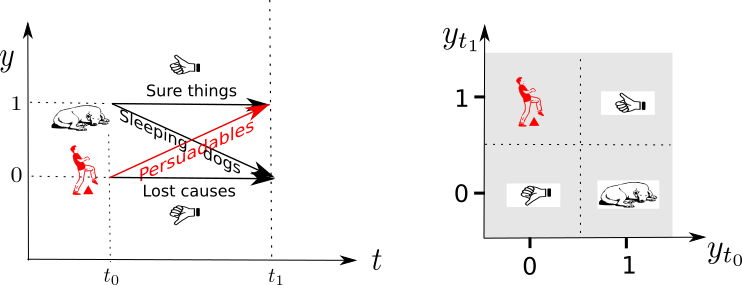
\includegraphics[width=6in]
{uplift/uplift-y-t.png}
\caption{UP diagnostic test
can be used to classify
all participants of the
population into 4 UP-types.
This figure 
assumes $y\in \bool$.
More generally, $y\in \RR$.
$t$ represents time. $t=t_0$
corresponds to $d=0=untreated$,
and $t=t_1$ corresponds to $d=1=treated$.} 
\label{fig-uplift-y-t}
\end{figure}

Let $y^B_t\in \RR$ for $t=t_0, t_1$
be the treatment response at time $t$
for participant $B$. (We are using here
the same notation as in Chapter \ref{ch-po}).
Call $\delta^B=
y^B_{t_1}-y^B_{t_0}$ the {\bf participant uplift}
for participant $B$.
As shown
in Fig.\ref{fig-uplift-y-t},
UP classifies participants
into 4 {\bf UP-types}: Persuadables, SureThings, LostCauses,
and SleepyDogs.
The UP-type
of a participant
depends on the changes 
that are induced on that participant
by an {\bf UP-diagnostic-test}.
\begin{itemize}
\item
For a {\bf Persuadable} participant,
$\delta^B>0$.
\item
For a {\bf SleepyDogs}
participant, $\delta^B< 0$.
\item
For a {\bf SureThings} participant,
 $\delta^B\approx 0$
and $y^B_{t_0}$ is high.
\item
For a {\bf LostCauses} participant,
$\delta^B\approx 0$
and $y^B_{t_0}$ is low.
\end{itemize}


Suppose $B$
belongs to
stratum $A_x$.
What is commonly called 
the {\bf uplift} 
is the {\bf stratum-uplift} $\delta_x=SDO$.
Strata can also be
classified into
the 4 UP-types,
depending on the sign and size  
of their $\delta_x$.
A participant 
may not be typical for
his stratum
and may
have different
{\bf participant and stratum UP-types}.
For example, he may have positive 
participant uplift
and therefore have a Persuadable participant UP-type,
but his stratum-uplift
might be negative, so
he has
the SleepyDogs stratum UP-type.

Advertisers are very interested in finding
the Persuadable strata in a population
so as to focus their resources on them.
For example, UP was used very
successfully during the 
Obama presidential campaigns. 
Team Obama conducted UP-diagnostic
tests much like
the climate change one described earlier.
This allowed them to
identify voters who might be sitting on the fence
on whether to vote for Obama or not.
Then Team Obama spent
the lion share
of  resources  on those
fence-sitters.


\section{Some Relevant Technical Facts from Chapter \ref{ch-po}}
Some relevant technical facts
about SDO
that were proven in Chapter \ref{ch-po} are

\begin{itemize}
\item
$SDO=0$ is the hypothesis tested 
by a Randomized Clinical Trial (RTC). 

\item
Using $\rvy=\rvy(\rvtd)$
and Fig.\ref{fig-y-diffs-square-probs},
we get

\beqa
SDO &=& \sum_y y\left[
P_{\rvy(1)|\rvtd, \rvx}(y|1, x)
-
P_{\rvy(0)|\rvtd, \rvx}(y|0, x)
\right]
\\
&=&
\sum_y y\left[
P_{\rvy|\rvtd, \rvx}(y|1, x)
-
P_{\rvy|\rvtd, \rvx}(y|0, x)
\right]
\;.
\eeqa
If $\rvy\in \bool$, then

\beq
\underbrace{SDO}_{\displaystyle \delta_x}
=
\underbrace{
P_{\rvy|\rvtd, \rvx}(1|1, x)
}_{\displaystyle Y^1_x}
-
\underbrace{
P_{\rvy|\rvtd, \rvx}(1|0, x)
}_{\displaystyle Y^0_x}
\;.
\eeq

\item
Recall that in
Chapter \ref{ch-po}, we used 
$A_{d, x}=\{\s:\td^\s=d,x^\s=x\}$,
$A_x=A_{0,x}\cup A_{1,x}$ and $A=\cup_x A_x$; also
$N_{d,x}=|A_{d,x}|$, $N_x=|A_x|$ and $N=|A|$.
From
Eq.(\ref{eq-est-sdo}),
we get


\beq
\underbrace{\widehat{SDO}}_{\displaystyle\delta_x}
=
\underbrace{\frac{1}{N_{1,x}}
\sum_{\s\in A_{1,x}} y^\s}_
{\displaystyle Y_x^1}
-
\underbrace{\frac{1}{N_{0,x}}
\sum_{\s\in A_{0,x}}  y^\s}_
{\displaystyle Y_x^0}
\;.
\label{eq-est-sdo-uplift}
\eeq

\end{itemize}


\section{UP Analysis}
\label{sec-up-analysis}

The input
to UP is a PO
dataset $DS= \{ (\s, d^\s, x^\s, y^\s):
 \s=0,1, 2, \ldots, nsam-1\}$.
where $d^\s\in \bool$, $x^\s \in S_\rvx$,
$y^\s\in \RR$.
A  participant $B$
is assigned two different
$\s$
if he/she
belongs to
both the treated and control groups.
We will assume 
$S_\rvx$ is a finite set.
In general,
$x=(x_0, x_1,\dots, x_{n-1})$ is an $n$ dimensional 
vector of features $x_i$.
If any of the $x_i$
is a priori continuous, we will
assume it has  been binned into
a finite number of bins.

\begin{figure}[h!]
\centering
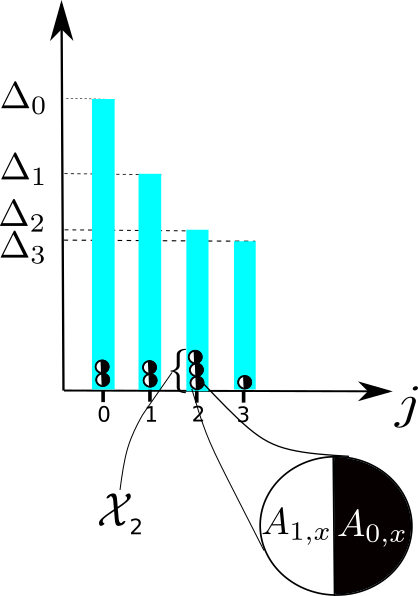
\includegraphics[width=2in]
{uplift/uplift-bins.png}
\caption{
Pictorial
representation
of the sequence
$\{(\calx_c, \Delta_c)\}_{c=0,1, \ldots, nc-1}$.
}
\label{fig-uplift-bins}
\end{figure}


Starting with $DS$,
UP performs the following steps.
Fig.\ref{fig-uplift-bins}
is a pictorial representation
of the quantities
that are calculated
during these steps.

\begin{enumerate}
\item Find $A_x$ 
for each observed $x\in S_\rvx$.
Set $A_x=\emptyset$ for unobserved $x\in S_\rvx$.
 
\item Calculate $\delta_x$
for each $x\in S_\rvx$.
Set $\delta_x=0$ if $A_x=\emptyset$.

\item Calculate
the set 

\beq\{\Delta_c\}_{c=0, 1, \ldots, nc-1}=
\{\delta_x: x\in S_\rvx\}
\eeq
of distinct uplifts $\delta_x$.
The class labels 
$c$ should be assigned
so that the sequence of
$\Delta_c$
is monotonic and non-increasing; i.e.,

\beq
\Delta_0 \geq \Delta_{1}\geq\cdots \geq \Delta_{nc-1}
\;.
\eeq
Now calculate 

\beq
\calx_c =\{ x: \delta_x =\Delta_c\}
\eeq
 for each $c$.
By the end of this step,
we will have calculated 
$\{(\calx_c, \Delta_c)\}_{c=0,1, \ldots, nc-1}$.
We will refer to the $\calx_c$
as {\bf strata-bins}. Note that
\beq
\Delta_c = 
\underbrace{\frac{1}{|\calx_c|}\sum_{x\in\calx_c}Y^1_x}_
{\displaystyle Y^1_c}
- 
\underbrace{\frac{1}{|\calx_c|}\sum_{x\in\calx_c}Y^0_x}_
{\displaystyle Y^0_c}
\;.
\label{eq-Delta-c}
\eeq
\item
For each $c$,
calculate 

\beq
\Sigma_{d,c}=\cup_{x\in \calx_c}A_{d,x}
\eeq
for $d\in\bool$
and 

\beq
\Sigma_{c}=\Sigma_{0,c}
\cup \Sigma_{1,j}
\;.
\eeq
\end{enumerate}


\begin{figure}[h!]
\centering
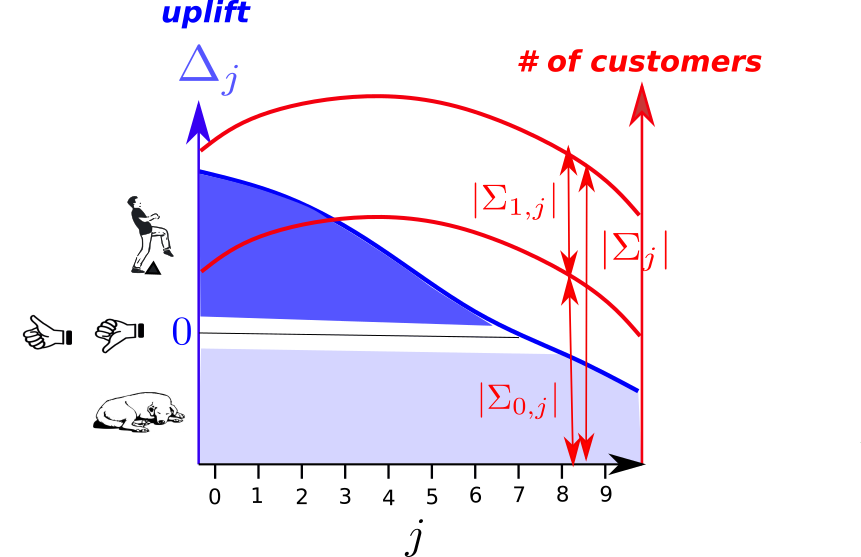
\includegraphics[width=4in]
{uplift/qini-fake.png}

\caption{
Plot
of UP results.
Alternative to Qini curves.
} 
\label{fig-qini-fake}
\end{figure}
Fig.\ref{fig-qini-fake}
is a  way of
plotting
the results 
of UP in an
intuitive
way
that even a
business type can understand.
UP software
often plots something
called a Qini
curve, 
but I find Qini
curves opaque, confusingly defined 
in the literature, unnecessary
and 
not very well motivated. So I don't
use or recommend them.




\section{UP Decision Trees}

In this section,
we will describe
how to build UP decision trees (UP dtrees),
and explain why they are needed
for UP.
Generic dtrees are 
described in Chapter \ref{ch-dtree}.
This section 
complements rather than replaces
that chapter so the reader
is advised to read
that chapter first.
Ref.\cite{jaros} is an excellent paper on the use of
dtrees in UP.

The
analysis described
previously in  
Section
\ref{sec-up-analysis},
although theoretically correct,
will work very poorly in practice.
 The strata-bins
of Section
\ref{sec-up-analysis}
correspond to
the classification
classes of a dtree.
But strata-bins are very
specific so they  
severely overfit the data.
Although dtrees 
can also suffer from overfitting,
there are known methods of 
preventing or mitigating overfitting in dtrees.
There are also tasks 
that dtrees 
can do well
and the methods
explained so far
cannot do well.
For example,
suppose we have 
a classless
dataset $DS^-=\{(\s, x^\s):\s\in \Sigma^-\}$
and we want to predict
the class $c^\s$ and
uplift $\Delta_{c^\s}$
for each of these individuals 
$\s\in \Sigma^-$.
A dtree can easily
do that. The alternative
is to use the classy dataset 
$DS=\{(\s, x^\s, c^\s):\s\in \Sigma\}$
to
prepare a dictionary
that orders
the elements
of $S_\rvx$ and gives a
class $c$ and an uplift value
$\Delta_c$ for each
feature vector $x\in S_\rvx$.
But
such a dictionary overfits
and says nothing for 
feature vectors $x$
that do not show up in 
the classy dataset $DS$; i.e., the
dictionary 
doesn't guess (interpolate). Dtrees,
on the other hand, do
guess.

So, without further ado,
let us describe how to
modify the results
of Chapter \ref{ch-dtree}
on generic dtrees
to the case of UP dtrees.
The main difference,
as we will
explain in detail
next,
is that the Information
Gain metric
used for generic dtrees
needs to be replaced
by another metric.






\begin{figure}[h!]
$$
\xymatrix{
&\rvx_{k'}
\\
\rvx_j\ar[r]_{\rvx_j=x_j}
\ar[ru]^{\rvx_j=x_j'}&\rvx_k
\\
\{N^d_j(c)\}_{c\in S_\rvc}
&
\{N^d_k(c)\}_{c\in S_\rvc}
\\
\sum_{c\in S_\rvc}N^d_j(c)=N^d_j
&
\sum_{c\in S_\rvc}N^d_k(c)=N^d_k
\\
&
\sum_{k\in ch(j)}N^d_k(c)=N^d_j(c)
}
$$
\caption{Fig.\ref{fig-dtree-notation}
 with $d$ dependence added.
$d\in \bool$
is the treatment dose.
} 
\label{fig-dtree-notation-uplift}
\end{figure}

\begin{figure}
$$
\xymatrix{
\rvd\ar[dr]\ar[drr]
\\
\rvj
\ar[r]
&
\rvk\ar[r]
&
\rvc
}$$
\caption{Bnet derived from population
numbers in Fig.\ref{fig-dtree-notation-uplift}}
\label{fig-class-bnet-uplift}
\end{figure}



Fig.\ref{fig-dtree-notation-uplift}
was obtained from Fig.\ref{fig-dtree-notation}
in Chapter \ref{ch-dtree}
by adding $d$ dependence.
$d\in \bool$
is the treatment dose.
Since $d\in \bool$,
in UP, we build two dtrees
of the type that were built
in Chapter \ref{ch-dtree}
(both with the same structure
but with different 
probabilities associated with each 
node).
$N^d_j(c)$ is 
the number
of individuals $\s$
in the population that reaches node $\rvx_j$
with $d\in \bool$ and belonging
to class $c\in S_\rvc$. 
From these population numbers, we can define
the bnet in Fig.\ref{fig-class-bnet-uplift}.
The TPMs, printed in blue,
for the (non-root) nodes of this bnet, are as follows



\beq\color{blue}
P(c|k,d)=
\frac{N_k^d(c)}
{N_k^d}
\label{eq-p-c-pre-laplace}
\eeq

\beq\color{blue}
P(k|j, d)=
\frac{N_k^d}
{N_j^d}\indi(k\in ch(j))
\eeq


In Chapter
\ref{ch-dtree},
we used Information 
Gain
(a mutual information)
as the SAM (Separation Ability Measure)
in
SL (Structure Learning) 
of dtrees (Decision Trees).
Information Gain
is not an ideal
SAM for SL of UP dtrees,
because UP trees
have a more
specialized classification goal
than the generic dtrees of Chapter \ref{ch-dtree}.
Both UP trees and generic trees
want to
separate the sample
population into classes,
but the classes for an UP dtree 
are specifically uplift bins (i.e., uplift intervals).


Ref.\cite{jaros}
proposes and studies 
the following
3 SAMs. These SAMs 
are more efficient than
Information Gain
for SL of UP dtrees.


\begin{enumerate}
\item{\bf SAM\_DD} (DD=Delta Delta)

For $d\in \bool$
and $c, c'\in S_\rvc$, define the increments

\beq
\partial_d f(d)=f(1)-f(0)
\eeq
and

\beq
\partial_{c',c} f(c)=f(c')-f(c)
\;.
\eeq
Let

\beqa
\Delta_{c|j} &=& P(c|j,1)-P(c|j,0)
\\
&=& \partial_d P(c|j,d)
\label{eq-delta-c-j}
\eeqa

\beqa
SAM\_DD_j&=& \max_{c,c'}|\partial_{c',c}\partial_d P(c|j,d)|
\\
&=&
\max_{c,c'}|\partial_{c',c}\Delta_{c|j}|
\eeqa

\item{\bf SAM\_KL} (KL=Kullback Liebler)
\begin{align}
SAM\_KL_j&=
\left[
\sum_{k\in ch(j)}
P(k|j)
D_{KL}(P_{\rvc|k,1}\parallel P_{\rvc|k,0})
\right]
-
D_{KL}(P_{\rvc|j,1}\parallel P_{\rvc|j,0})
\\
&=
\left[
\sum_{k\in ch(j)}
P(k|j)
 \sum_{c\in S_\rvc}P(c|k,1) 
\ln \frac{P(c|k,1) }{ P(c|k,0) }
\right]
-
\sum_{c\in S_\rvc} 
P(c|j,1) 
\ln \frac{P(c|j,1) }{ P(c|j,0) }
\label{eq-sam-kl}
\end{align}

{\bf $SAM\_KL_j$ can be negative.}

\item {\bf SAM\_E} (E=Euclidean)

$SAM\_E$ is defined the same way as $SAM\_KL$
except with 
the KL divergence $D_{KL}(P\parallel Q)$ 
in $SAM\_KL$ replaced 
by the Euclidean distance squared. 


\beq
D(P,Q) =\sum_x (P(x)-Q(x))^2
\eeq

\end{enumerate}

The intuitive reason for
 using these quantities as
SAMs is that they maximize the change in uplift 
between 
successive tree levels, so 
that the uplift increases as quickly as possible
as we descend down the UP tree.
In the case of generic dtrees
for which we use Information Gain as SAM, we 
are maximizing the correlation
between classes and nodes as we descend down the tree. 
These two goals are related.
In fact, in the limit
where the
number of control individuals
becomes zero,
$SAM\_KL_j$ and $INFO\_gain_j$
become the same, as will be shown later.

Next we show
that $SAM\_KL_j$
satisfies the following 3
axioms\footnote{
We won't show it
here, but 
according to Ref.\cite{jaros},
$SAM\_E_j$ also satifies these
3 axioms, but
$SAM\_DD_j$
satisfies only the first two.}

\begin{claim}
.\newline
\begin{enumerate}
\item \label{item-sam-min}
$SAM\_KL_j$ 
is minimum
iff 
$P(c|k,0)=P(c|k, 1)$ 
for all $c$
and $k\in ch(j)$.
\item \label{item-sam-zero}
If $P(c|j,d)=P(c|d)$
for all $c,j,d$, then $SAM\_KL_j=0$.
\item
\label{item-no-control}
Suppose $N^0_j=0$ for all nodes $j$
 (i.e., no control population)
and we use the Laplace Correction
when warranted. Then

\begin{align}
SAM\_KL_j
&=
H(\rvc:\rvk|j,1)
\\
&=
INFO\_gain_j\;\;\; \text{ for treated population}
\;.
\end{align}
\end{enumerate}
\end{claim}
\proof

The proof of items
\ref{item-sam-min}
and \ref{item-sam-zero}
follow by inspection of Eq.\ref{eq-sam-kl}.
Item \ref{item-no-control}
is proven in Claim \ref{claim-no-control}
below.
\qed



Let $N_\rvc=|S_\rvc|$.
Define the uniform probability 
distribution 

\beq
U_\rvc(c)=\frac{1}{N_\rvc}
\eeq
for all $c\in S_\rvc$.

Eq.(\ref{eq-p-c-pre-laplace})
for the TPM of node
$\rvc$ in the bnet Fig.\ref{fig-class-bnet-uplift} can be
"Laplace Corrected"
as follows
so that it is no longer
undefined when
its denominator vanishes:

\beq
P(c|j,d)=
\left\{
\begin{array}{ll}
\frac{N^d_j(c)}
{N^d_j}&\text{ if } N^d_j>0
\\
U_\rvc(c) & \text{ if $N^d_j=0$ (Laplace Correction)}
\end{array}
\right.
\eeq




\begin{claim}
\label{claim-no-control}
Suppose $N^0_j=0$ for all dtree nodes $j$
and we use the Laplace Correction
when warranted. Then

\beq
SAM\_KL_j=H(\rvc:\rvk|j,1)
\;.
\eeq
\end{claim}
\proof

For all nodes $j$, we  must have

\beq
P_{\rvc|j,0}=U_\rvc
\eeq
so

\beqa
D_{KL}(P_{\rvc|j,1}\parallel P_{\rvc|j,0})
&=&
D_{KL}(P_{\rvc|j,1}\parallel U_\rvc)
\\
&=&
\ln(N_\rvc) - H(\rvc|j,1)
\;.
\label{eq-kl-reduce}
\eeqa
For all $k\in ch(j)$, we must also have


\beq
N_j=N_j^1,  N_k=N^1_k
\eeq
so

\beq
P(k|j)=
P(k|j,1)
\;.
\label{eq-p-kj-add-1}
\eeq
Now using Eqs.(\ref{eq-kl-reduce}) and
 (\ref{eq-p-kj-add-1}), we get


\beqa
SAM\_KL_j&=&
-\left[
\sum_{k\in ch(j)}
P(k|j)
H(\rvc|k,1)
\right]
+
H(\rvc|j,1)
\\
&=&
-\left[
\sum_{k\in ch(j)}
P(k|j,1)
H(\rvc|k,1)
\right]
+
H(\rvc|j,1)
\\
&=&
-H(\rvc|\rvk,j,1)+H(\rvc|j,1)
\;\;\;\text{(using  Claim \ref{claim-H-spliting})}
\\
&=&
H(\rvc:\rvk|j,1)
\eeqa
\qed


\subsection{Appendix, 
connection between
$\Delta_c$
and $\Delta_{c|j}$}

Recall Eq.\ref{eq-Delta-c}:

\beqa
\Delta_c &=& 
\underbrace{\frac{1}{|\calx_c|}\sum_{x\in\calx_c}Y^1_x}_
{\displaystyle Y^1_c}
- 
\underbrace{\frac{1}{|\calx_c|}\sum_{x\in\calx_c}Y^0_x}_
{\displaystyle Y^0_c}
\\
&=&
\partial_d Y^d_c
\;.
\eeqa
Compare that to Eq.(\ref{eq-delta-c-j}):
\beqa
\Delta_{c|j} &=& P(c|j,1)-P(c|j,0)
\\
&=& \partial_d P(c|j,d)
\eeqa
What is the connection
between these 2 deltas, $\Delta_c$
and $\Delta_{c|j}$? Are they equal?

First off, notice that 
$\Delta_{c|j}$ is defined for all 
nodes $j$ of the dtree. Let 
$j(c)$ be the leaf node 
for which $\Delta_c\approx \Delta_{c|j(c)}$. 
Assume $y^\s\in\bool$. Then

\beq
P(c|j=j(c), d)=\frac{N^d_{j(c)}(c)}{N^d_{j(c)}}
\approx Y^d_c
\eeq
So the two deltas are indeed approximately equal
when $y^\s\in \bool$ and $j=j(c)$.

